\subsection{Backend megvalósítása}

\subsubsection{Adathozzáférési réteg - DAL}

\textbf{Eloquent ORM:}
A backenden, a Laravel keretrendszerben az adathozzáférési réteget az Eloquent nevezetű ORM (Object Relational Mapper) biztosítja. Az Eloquent segítségével a PHP objektumokat és az adatbázis táblákat lehet egymáshoz kapcsolni. Az Eloquent ORM segítségével lehetőség van migrációk írására, modellek, seeder-ek, factory-k, stb. létrehozására.\\

\textbf{Migrációk:}
A migrációs fájlok segítségével a táblák struktúráját lehet definiálni. Ez különösen hasznos a hordozhatóság szempontjából, mivel a migrációk segítségével a fejlesztők könnyen telepíthetik az alkalmazást a különböző adatbáziskezelőket használó környezetekbe. Mi a backend fejlesztése során a MySQL adatbázist használtunk.

Külön kiemelendő, hogy a Laravelben lehetőség nyílik UUID-k haználatára integer ID-k helyett amit ki is használtunk. Ennek előnye, hogy ez egy 36 hosszú alkalmazás szinten egyedi szöveges azonosítót generál minden rekordhoz, így kevésbé kikövetkezethető az adatbázis tartalma, mely nagyobb biztonságot nyújt. A globális egyediség az ütközések elkerülése végett is előnyös.\\ 

\textbf{Modellek:}
A modellek az táblákat reprezentálják az alkalmazásban objektum orientált módon, ahol maga az osztály a tábla, az osztály példányok pedig a tábla sorai. A modellek segítségével lehetőség van az adatok lekérdezésére, frissítésére, törlésére, valamint az adatok közötti kapcsolatok definiálására, így az 1:1 kapcsolatok, 1:N kapcsolatok, N:M kapcsolatok is könnyen definiálhatóak.

Ezen kívűl a Like és Comment modelleknél a beépített Morph relációkat is használtuk, melyek segítségével egy táblához több másik tábla is kapcsolódhat (polymorphic relationship). Ehhez a Laravel minden táblához egy \textit{\_type} és egy \textit{\_id} mezőt ad hozzá (pl: \texttt{likeable\_type} és \texttt{likeable\_id}), melyek segítségével azonosítani lehet a kapcsolódó táblát és azon belül az egyedi azonosítót.

Az alkalmazásunkban található modellek áttekintő ábrája a \ref{fig:models}. ábrán látható.

\begin{figure}[H]
    \centering
    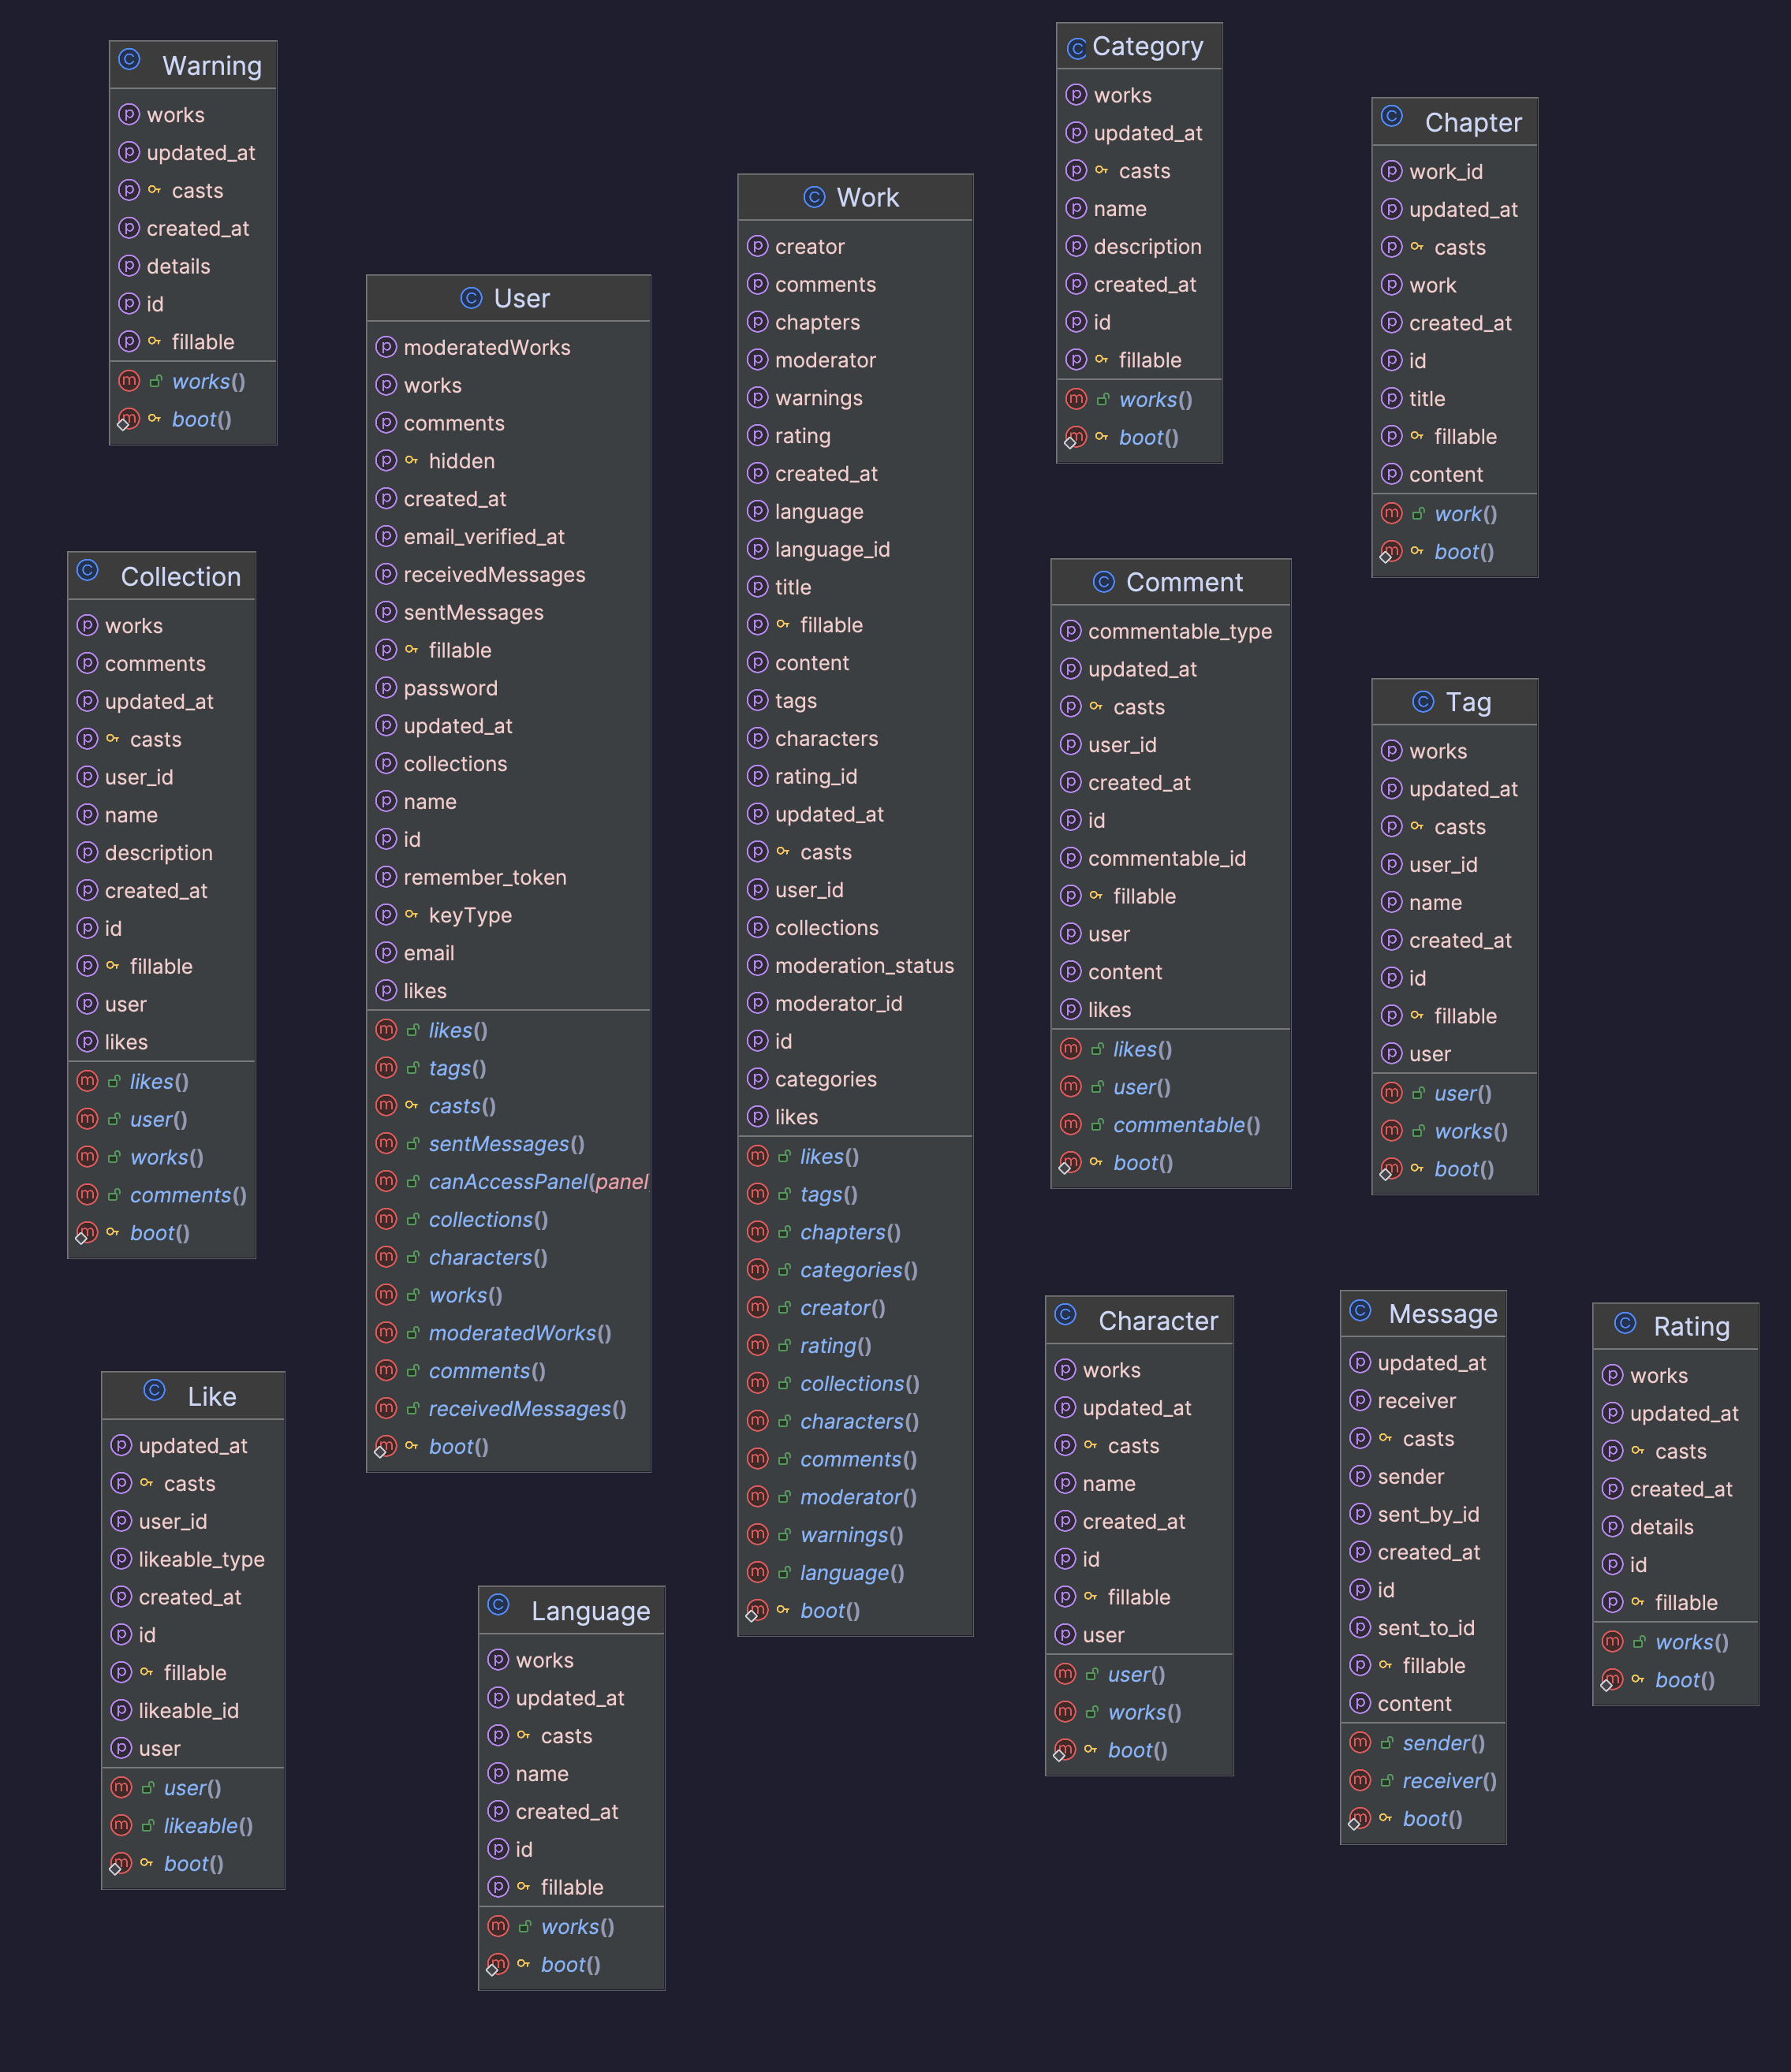
\includegraphics[scale=0.1]{./figures/models.png}
    \caption{Az alkalmazás modelljei}
    \label{fig:models}
\end{figure}


\textbf{Factory-k:}
A factory-k segítségével lehetőség van tesztadatok generálására az adatbázisba. A factory-k segítségével lehetőség van a modellekhez kapcsolódó adatok generálására, amelyeket a tesztelés során lehet használni. Ehhez a Laravel a Faker nevű könyvtárat használja, amely segítségével különböző típusú hamis, de struktúrális tekintetben helytálló adatokat lehet generálni.\\

\textbf{Seeder-ek:} A factory osztályok segítségével generált adatokat a seeder-ek segítségével lehet az adatbázisba betölteni, meghatározott mennyiségben és kapcsolatokkal. Külön jelentősége volt a \texttt{PermissionSeeder}-nek mely az alkalmazás jogosultságait definiálja.\\

\subsubsection{Üzleti logika réteg - BLL}


\textbf{Authentikáció:} Az authentikációra a Laravel Breeze csomagot használtuk, mely egy minimális authentikációs rendszert biztosít. Az authentikációhoz szükséges routokat, controllereket, view-kat és middleware-eket a csomag automatikusan generálja. Az authentikációhoz szükséges adatbázis táblákat is a csomag generálja, így a felhasználók regisztrációja, bejelentkezése, jelszó visszaállítása, stb. egyszerűen megvalósítható.

A Breeze alapvetően Session alapú CSRF és CORS védelemmel rendelkező authentikációt biztosít a frontendek számára. Azonban maga a Breeze egy másik csomagra a Laravel Sanctum-ra épít. Ennek előnye, hogy a Sanctum biztosít API Token alapú authentikációt is melyet a mobil kliens így ki tudott használni.\\

\textbf{Authorizáció:} Az authorizációra a Spatie cég által fejlesztett és karbantartott Laravel Permission csomagot használtuk. A csomag segítségével lehetőség van jogosultságok (permissions) definiálására, azokhoz szerepkörök (roles) rendelésére, valamint a jogosultságok és szerepkörök alapján az authorizáció megvalósítására. A csomag a Laravel Policy-ket használja az authorizáció megvalósítására, amelyek segítségével a jogosultságokat és szerepköröket a modellekhez lehet rendelni.

Ennek előnye hogy ellenőrzéskor csak a jogosultság meglétét kell ellenőrizni, azonban a jogosultságok egységesen kioszthatók role-ok segítségével. Az alkalmazás 3 szerepkört valósít meg, melyek a \texttt{Registered}, \texttt{Moderator} és \texttt{Admin}. Az admin az alkalmazás ServiceProvider-ében minden ellenőrzésen automatikusan átengedésre kerül, így nem kell az össze jogosultságot hozzárendelni.\\

\subsubsection{Tesztelés}

Teszteltünk, PEST, mekkora fedettség, mi lett tesztelve és miért

\subsubsection{Admin felület}

Bár nem külön alkalmazás réteg de megemlítendő, hogy az admin felület megvalósítására a FilamentPHP csomagot használtuk a backend oldalon. Előnye, hogy a modell osztályokhoz definiálhatóak úgynevezett filament resource-ok melyek az admin felületen megjelenő mezőket és azok viselkedését definiálják. A csomag segítségével lehetőség van a modellek szerkesztésére, törlésére, listázására, stb. Az admin felület a \ref{fig:admin}. ábrán látható.

\begin{figure}[H]
    \centering
    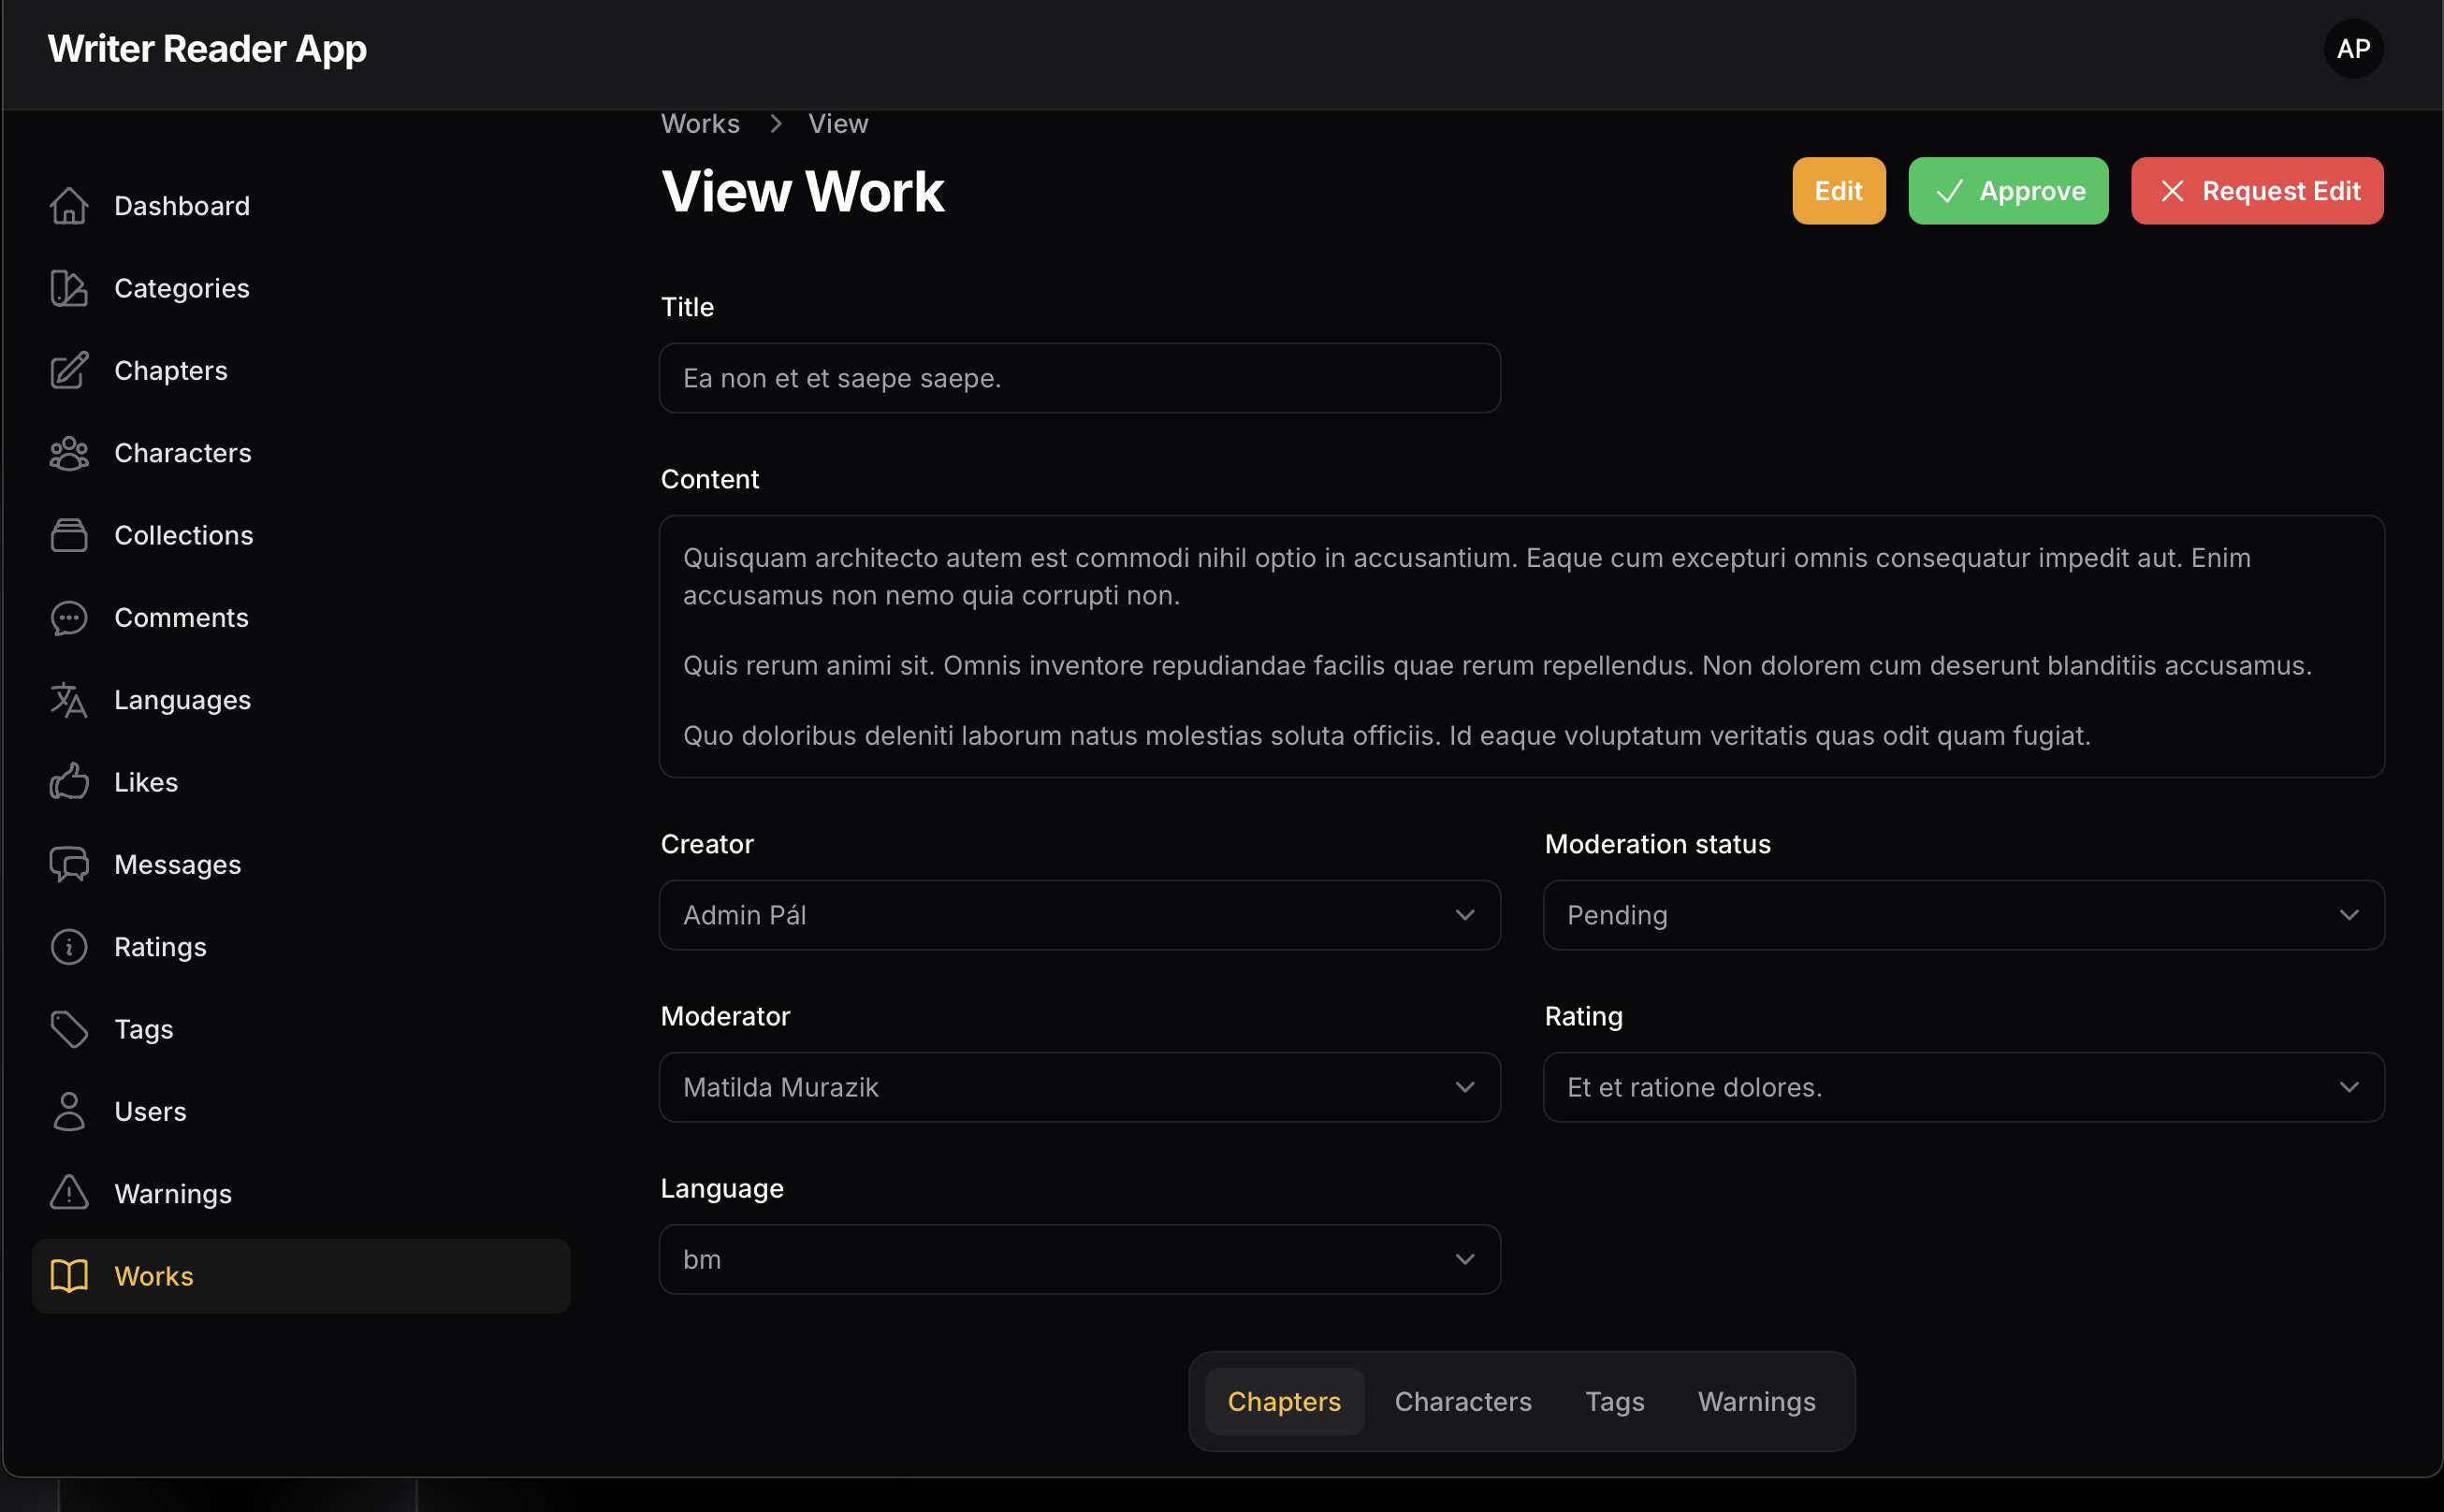
\includegraphics[scale=0.25]{./figures/admin-panel.png}
    \caption{FilamentPHP admin felület}
    \label{fig:admin}
\end{figure}

Az admin felülethez csak moderátor és admin jogosultságú felhasználó férhet hozzá. Azon belül az egyes modellek-hez való hozzáférést a policy osztályok szabályozzák de felülírható külön a filament resource-okon keresztül is.

Ezen kívűl az adminfelületen került megvalósításra a művek jóváhagyása is melyekre a moderátoroknak van jogosultságuk. A jóváhagyás után a művek publikussá válnak és megjelennek a felhasználók számára is, valamint automatikusan email értesítés küldődik a mű létrehozójának.